\chapter{Elettromagnetismo}

\section{Esercizio 1}

\subsection{Prima domanda}

\begin{center}
  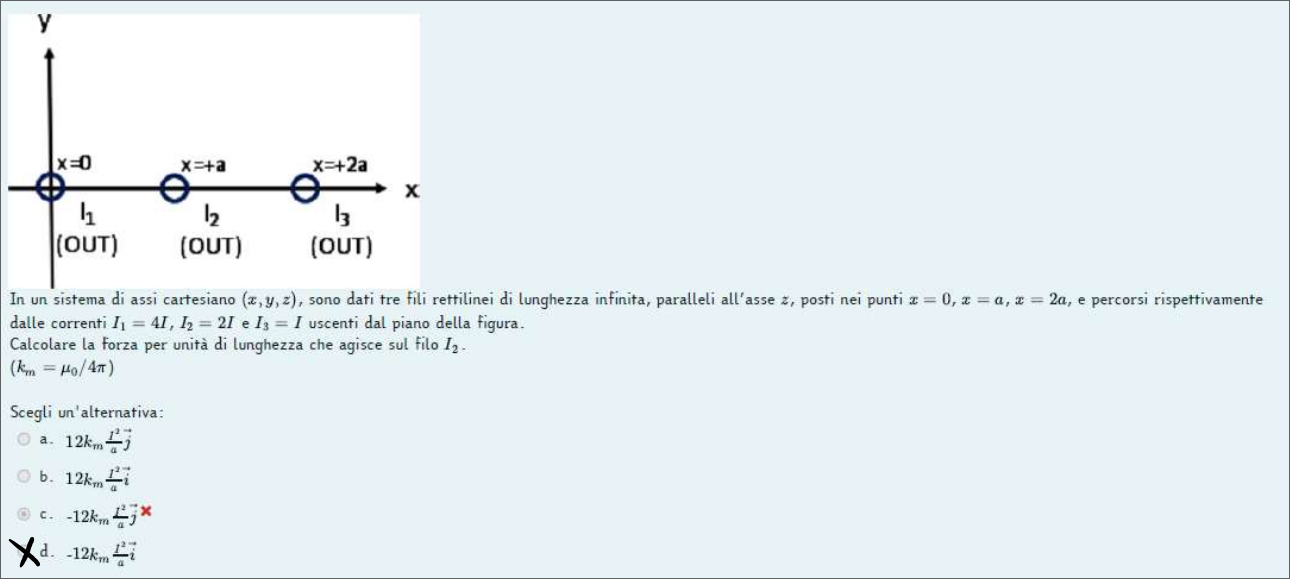
\includegraphics[scale=0.35]{es1-1em.png}
\end{center}

\paragraph{Risposta:} si usa la regola della mano destra per stabilire se il contributo apportato sia positivo o negativo. In questo caso si nota che $I_1$ apporta un contributo positivo a $I_2$, mentre il contributo di $I_3$ è negativo. Si prosegue facendo la somma delle due forze ottenute dalla formula $2k_m \frac{I_a I_b}{d}$ e il versore è "$\vec{i}$" perchè il contributo si ha sull'asse delle x.

$$F_T = F_{1-2} - F_{2-3} = 2k_m (\frac{I 2I}{a} - \frac{2I 4I}{a}) \vec{i} = 2k_m (-\frac{6I^2}{a}) \vec{i} = 12k_m \frac{I^2}{a} \vec{i}$$

\subsection{Seconda domanda}

\begin{center}
  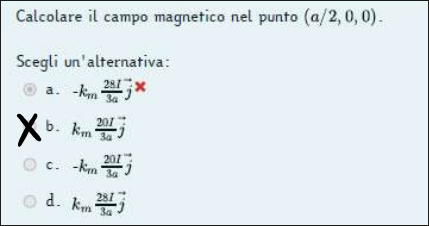
\includegraphics[scale=0.5]{es1-2em.png}
\end{center}

\paragraph{Risposta:} si applica un procedimento simile al precedente esercizio. In questo caso il punto è a metà tra $I_1$ e $I_2$ quindi, applicando la regola della mano destra si sa che $I_1$ è positivo, mentre $I_2$ e $I_3$ sono negativi. Si usa la formula per il campo magnetico: $2k_m\frac{I}{r}$. La distanza è $\frac{a}{2}$ per $I_1$ e $I_2$, mentre $\frac{3a}{2}$ per $I_3$. Il contributo è $\vec{j}$ in quanto perpendicolare al campo magnetico. 

$$B_T = B_1 - B_2 - B_3 = 2k_m(\frac{4I}{\frac{a}{2}} - \frac{2I}{\frac{a}{2}} -\frac{I}{\frac{3a}{2}}) \vec{j} = 2k_m(\frac{8I}{a} - \frac{4I}{a} -\frac{2I}{3a}) \vec{j} = 2k_m (\frac{10}{3a}) \vec{j} = k_m \frac{20I}{3a} \vec{j}$$

\subsection{Terza domanda}

\begin{center}
  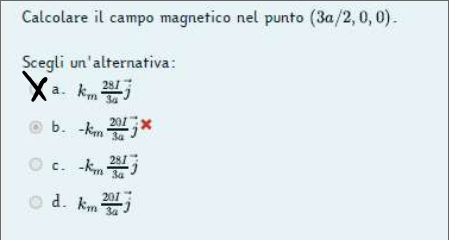
\includegraphics[scale=0.5]{es1-3em.png}
\end{center}

\paragraph{Risposta:} procedimento identico a quello dell'es precedente, ma sta volta sono $I_1$ e $I_2$ a essere positive.

$$B_T = B_1 + B_2 - B_3 = 2k_m(\frac{4I}{\frac{3a}{2}} + \frac{2I}{\frac{a}{2}} -\frac{I}{\frac{a}{2}}) \vec{j} = 2k_m(\frac{8I}{3a} + \frac{4I}{a} -\frac{2I}{a}) \vec{j} = 2k_m (\frac{14}{3a}) \vec{j} = k_m \frac{28I}{3a} \vec{j}$$

\subsection{Quarta domanda}

\begin{center}
  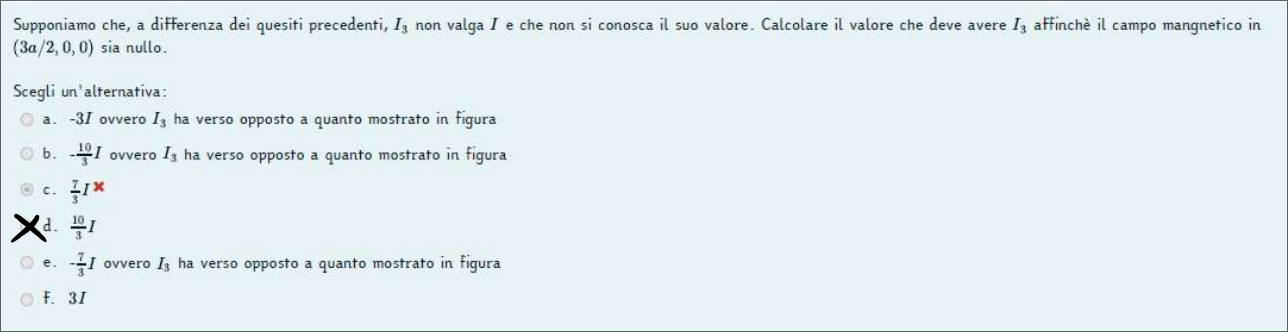
\includegraphics[scale=0.34]{es1-4em.png}
\end{center}

\paragraph{Risposta:} semplicemte si prende la somma della terza domanda e la si pone uguale a 0 sostituendo $I_3$ con $x$. 

$$\frac{8I}{3a} + \frac{4I}{a} -\frac{2x}{a} = 0 \rightarrow 8I + 12I - 6x = 0 \rightarrow 6x = 20I \rightarrow x = \frac{20I}{6} \rightarrow x = \frac{10I}{3}$$

\section{Esercizio 2}

\subsection{Prima domanda}

\begin{center}
  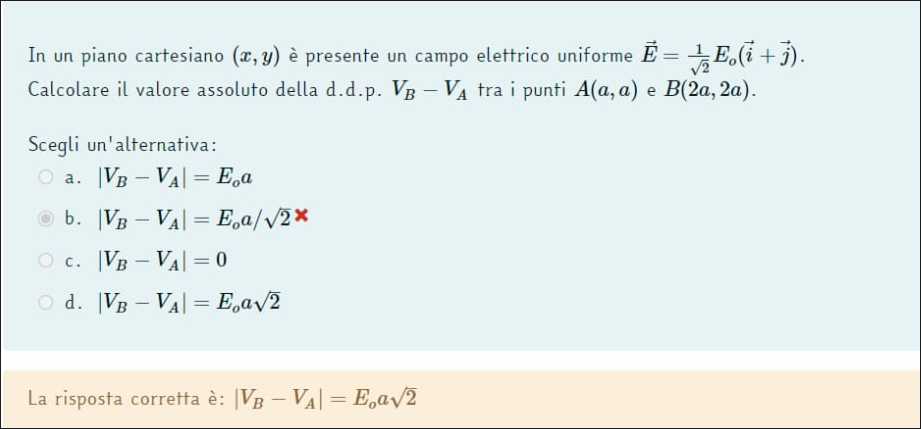
\includegraphics[scale=0.34]{es2-1em.png}
\end{center}

\paragraph{Risposta:} la differenza di potenziale calcola con $\delta V = \vec{E} S_{a\rightarrow b}$, dove $S_{a \rightarrow b}$ è lo spostamento da a a b. 

$$\Delta V = \frac{1}{\sqrt{2}} E_0 a \vec{i} + \frac{1}{\sqrt{2}} E_0 a \vec{j} =  \frac{2}{\sqrt{2}} E_0 a = E_0 a \sqrt{2}$$

\subsection{Seconda domanda}

\begin{center}
  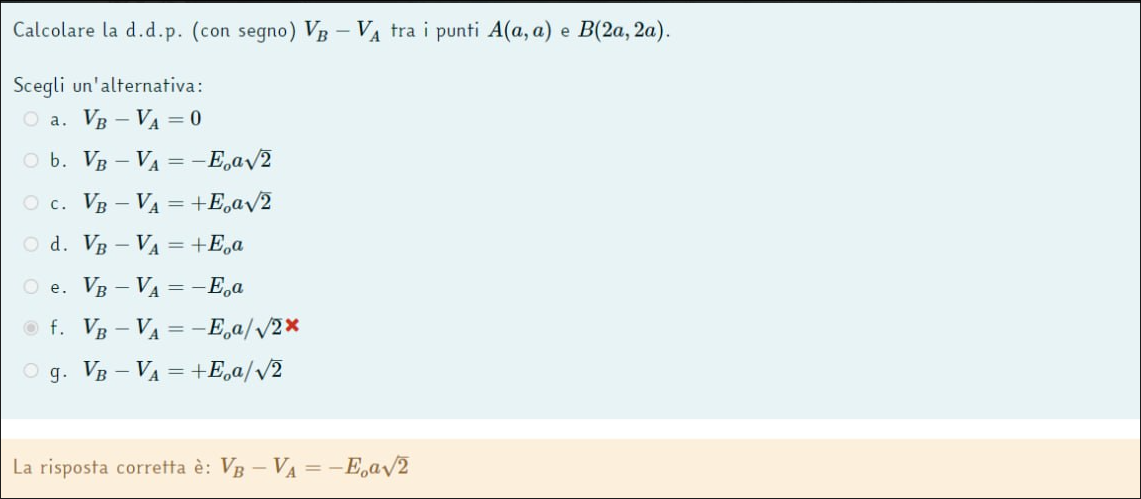
\includegraphics[scale=0.34]{es2-2em.png}
\end{center}

\paragraph{Risposta:} il segno è negativo perché si applica la regola della mano destra.

\subsection{Terza domanda}

\begin{center}
  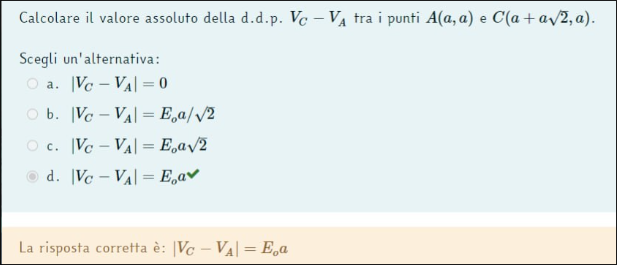
\includegraphics[scale=0.4]{es2-3em.png}
\end{center}

\paragraph{Risposta:} stesso ragionamento della prima domanda.

$$\Delta V = \frac{1}{\sqrt{2}} E_0 a \sqrt{2} = E_0 a$$

\subsection{Quarta domanda}

\begin{center}
  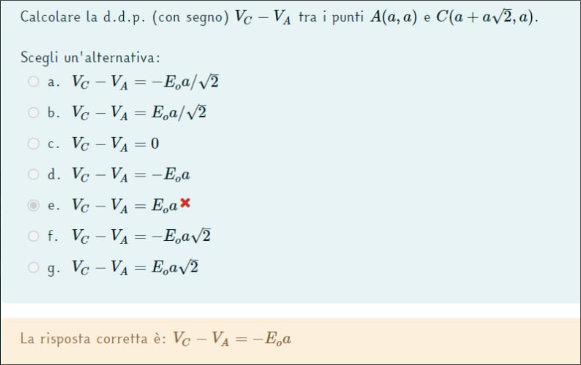
\includegraphics[scale=0.4]{es2-4em.png}
\end{center}

\paragraph{Risposta:} stesso ragionamento della seconda domanda.

\subsection{Quinta domanda}

\begin{center}
  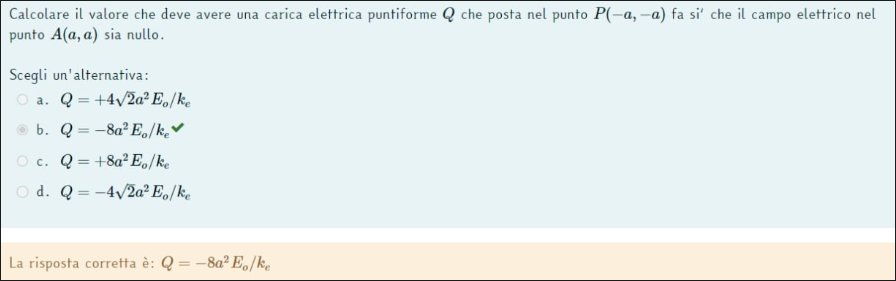
\includegraphics[scale=0.4]{es2-5em.png}
\end{center}

\paragraph{Risposta:} ???
